%%%%%%%%%%%%%%%%%%%%%%%%%%%%%%%%%%%%%%%%%%%%%%%%%%%%%%%%%%%%%%%%%%%%%%
\begin{frame}[fragile]\frametitle{}
\begin{center}
{\Large Graph}
\end{center}

\end{frame}

%%%%%%%%%%%%%%%%%%%%%%%%%%%%%%%%%%%%%%%%%%%%%%%%%%%%%%%%%%%%%%%%%%%%%
\begin{frame}
	\frametitle{Graph}
		\begin{itemize}
		\item Collection of nodes connected by edges
		\item Cycles are allowed.
		\end{itemize}
		
\begin{center}
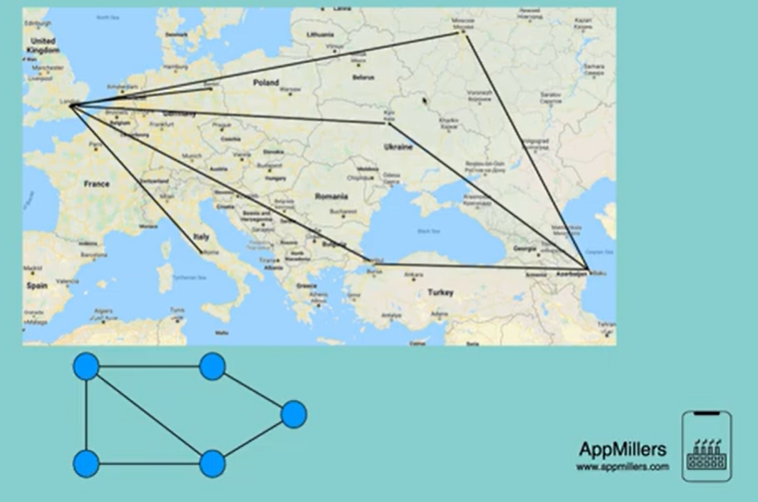
\includegraphics[width=0.8\linewidth,keepaspectratio]{graph6.png}
\end{center}

\end{frame}


%%%%%%%%%%%%%%%%%%%%%%%%%%%%%%%%%%%%%%%%%%%%%%%%%%%%%%%%%%%%%%%%%%%%%%
\begin{frame}
	\frametitle{A Graph}

	\begin{columns}[T]
		\column{0.5\linewidth}
		\begin{tikzpicture}[scale=0.8, transform shape]
	\begin{scope}[every node/.style={circle,thick,draw,onslide=<2>{draw=red}}]
    \node (A) at (0,0) {A};
    \node (B) at (0,3) {B};
    \node (C) at (2.5,4) {C};
    \node (D) at (2.5,1) {D};
    \node (E) at (2.5,-3) {E};
    \node (F) at (5,3) {F} ;
\end{scope}

\begin{scope}[>={Stealth},
              every node/.style={fill=white,circle},
							every edge/.style={very thick, draw=black,onslide=<3>{draw=red}}]
    \path (A) edge (B);
    \path (B) edge (C);
    \path (A) edge (D);
    \path (D) edge (C);
    \path (A) edge (E);
    \path (D) edge (E);
    \path (D) edge (F);
    \path (C) edge (F);
    \path (E) edge (F); 
    \path (B) edge[bend right=60] (E); 
\end{scope}
\end{tikzpicture}

		\column{0.5\linewidth}
		\begin{itemize}
			\item A graph is just a bunch of circles and lines.
				
			\item These circles are called \alert{vertices} (or \alert{nodes}).
				
			\item These lines are called \alert{edges} (or \alert{connections}).
				
			\item In this form the graph is called \textit{undirected} and \textit{unweighted}.
		\end{itemize}
	\end{columns}
\end{frame}

%%%%%%%%%%%%%%%%%%%%%%%%%%%%%%%%%%%%%%%%%%%%%%%%%%%%%%%%%%%%%%%%%%%%%%
\begin{frame}
	\frametitle{Directed Graphs}
	
	\begin{columns}[T]
		\column{0.5\linewidth}

					\begin{tikzpicture}[scale=0.8, transform shape]
	\begin{scope}[every node/.style={circle,thick,draw}]
    \node (A) at (0,0) {A};
    \node (B) at (0,3) {B};
    \node (C) at (2.5,4) {C};
    \node (D) at (2.5,1) {D};
    \node (E) at (2.5,-3) {E};
    \node (F) at (5,3) {F} ;
\end{scope}

\begin{scope}[>={Stealth},
              every node/.style={fill=white,circle},
							every edge/.style={draw=black,very thick}]
							\path[->] (A) edge (B);
							\path[->] (B) edge (C);
							\path[->] (A) edge (D);
							\path[->] (D) edge (C);
							\path[->] (A) edge (E);
							\path[->] (D) edge (E);
							\path[->] (D) edge (F);
							\path[->] (C) edge (F);
							\path[->] (E) edge (F); 
							\path[->] (B) edge[bend right=60] (E); 
\end{scope}
\end{tikzpicture}



		\column{0.5\linewidth}
		\begin{itemize}
			\item Edges can also have a direction.
			\item In which case we call it a \textit{directed} graph.

		\end{itemize}
		

	\end{columns}
\end{frame}

%%%%%%%%%%%%%%%%%%%%%%%%%%%%%%%%%%%%%%%%%%%%%%%%%%%%%%%%%%%%%%%%%%%%%%
\begin{frame}
	\frametitle{Directed Graphs}
	
	\begin{columns}[T]
		\column{0.5\linewidth}

			\begin{tikzpicture}[scale=0.8, transform shape]
\begin{scope}[every node/.style={circle,thick,draw}]
    \node (A) at (0,0) {A};
    \node (B) at (0,3) {B};
    \node (C) at (2.5,4) {C};
    \node (D) at (2.5,1) {D};
    \node (E) at (2.5,-3) {E};
    \node (F) at (5,3) {F} ;
\end{scope}

\begin{scope}[>={Stealth[black]},
              every node/.style={fill=white,circle},
              every edge/.style={draw=black,very thick}]
    \path [->] (A) edge node {$5$} (B);
    \path [->] (B) edge node {$3$} (C);
    \path [->] (A) edge node {$4$} (D);
    \path [->] (D) edge node {$3$} (C);
    \path [->] (A) edge node {$3$} (E);
    \path [->] (D) edge node {$3$} (E);
    \path [->] (D) edge node {$3$} (F);
    \path [->] (C) edge node {$5$} (F);
    \path [->] (E) edge node {$8$} (F); 
    \path [->] (B) edge[bend right=60] node {$1$} (E); 
\end{scope}
\end{tikzpicture}



		\column{0.5\linewidth}
		\begin{itemize}
			\item Furthermore they can have weights.
			\item In which case we call it a \textit{weighted} graph.
		\end{itemize}
		

	\end{columns}
\end{frame}


%%%%%%%%%%%%%%%%%%%%%%%%%%%%%%%%%%%%%%%%%%%%%%%%%%%%%%%%%%%%%%%%%%%%%%
\begin{frame}
	\frametitle{Let's formalise!}

A formal definition of a graph:
			\begin{itemize}
				\item A graph $G=(V,E)$, where:
					\begin{itemize}
						\item $V$ is a set of vertices,
						\item $E$ is a set of edges, where every edge has two \textit{endpoints}.
					\end{itemize}
					
				\item If the graph is \textit{weighted} then there is a function $w: E \to \mathbb{R}$ which maps every edge to
					a weight.
					
					\begin{itemize}
						\item In most cases we will restrict ourselves to functions $w: E \to \mathbb{N}$, i.e. non-negative integer weights.
					\end{itemize}
					
				\item Depending on direction:
					\begin{itemize}
					
						\item If the graph is \textit{directed} then every edge $e = (u,v)$ with $u,v \in V$. In this case we call
							$u$ the \textit{origin} and $v$ the \textit{destination}
					
				\item If the graph is \textit{undirected} then every edge $e = \{u,v\}$ with $u,v \in V$.
				\item Unfortunately in many textbooks/papers/slides people also use $e=(u,v)$ for undirected edges, but just remark they are
					undirected.
					\end{itemize}
			\end{itemize}
\end{frame}

%%%%%%%%%%%%%%%%%%%%%%%%%%%%%%%%%%%%%%%%%%%%%%%%%%%%%%%%%%%%%%%%%%%%%%
\begin{frame}
	\frametitle{Let's draw}

		Draw the following graph:
		\begin{itemize}
			\item $V = \{A,B,C,D,E,F\}$\\
			\item	$E = \{
			\{A, B\},
			\{A, D\},
			\{D, C\},
			\{B, F\},
			\{B, E\},$\\$
			\{E, D\},
			\{E, F\},
			\{C, F\},
			(A,C),
			(C,A),
			(D,B),
			(B,C)
		\}$\\
	\item $w(\{E,D\}) = 8$, $w((A,C)) = 2$, $w(\{C,F\}) = 5$, $w(\{E,B\}) = 2$, $w((C,A)) = 8$.
		For all other edges $e$, $w(e) = 1$.
		\end{itemize}
\end{frame}

%%%%%%%%%%%%%%%%%%%%%%%%%%%%%%%%%%%%%%%%%%%%%%%%%%%%%%%%%%%%%%%%%%%%%%
\begin{frame}
	\frametitle{Properties of vertices}
		
	\begin{columns}[T]
		\column{0.5\linewidth}
			\begin{tikzpicture}[scale=0.8, transform shape]
	\begin{scope}[every node/.style={circle,thick,draw}]
		\node[onslide=<2-3>{draw=red}] (A) at (0,0) {A};
    \node (B) at (0,3) {B};
    \node[onslide=<4-5>{draw=red}] (C) at (2.5,4) {C};
		\node[onslide=<2>{draw=red}] (D) at (2.5,1) {D};
    \node (E) at (2.5,-3) {E};
    \node (F) at (5,3) {F} ;
\end{scope}

\begin{scope}[>={Stealth},
              every node/.style={fill=white,circle},
							every edge/.style={draw=black,very thick}]
							\path[onslide=<4->{->}] (A) edge[onslide=<3>{draw=red}] (B);
							\path[onslide=<4->{->}] (B) edge[onslide=<4>{draw=red}] (C);
							\path[onslide=<4->{->}] (A) edge[onslide=<3>{draw=red}] (D);
							\path[onslide=<4->{->}] (D) edge[onslide=<4>{draw=red}] (C);
							\path[onslide=<4->{->}] (A) edge[onslide=<3>{draw=red}] (E);
							\path[onslide=<4->{->}] (D) edge (E);
							\path[onslide=<4->{->}] (D) edge (F);
							\path[onslide=<4->{->}] (C) edge[onslide=<5>{draw=red}] (F);
							\path[onslide=<4->{->}] (E) edge (F); 
							\path[onslide=<4->{->}] (B) edge[bend right=60] (E); 
\end{scope}
\end{tikzpicture}

		\column{0.5\linewidth}
		Vertices also have some properties:
		
		\begin{itemize}
			\item Two vertices are \alert{adjacent} if there is an edge between them.
			\item We also call these \alert{neighbouring} vertices.
				
			\item Every vertex has a set of \alert{incident} edges, namely those connected to it.
				
			\item If the graph is directed, we can split this into:
				\begin{itemize}
					\item \alert{incoming} edges.
						
					\item \alert{outgoing} edges.
				\end{itemize}
		\end{itemize}
	\end{columns}
\end{frame}

%%%%%%%%%%%%%%%%%%%%%%%%%%%%%%%%%%%%%%%%%%%%%%%%%%%%%%%%%%%%%%%%%%%%%%
\begin{frame}
	\frametitle{More formalization}
Properties of vertices:
		\begin{itemize}
			\item Two vertices $u,v \in V$ are adjacent, or neighbours, iff $\exists e \in E$ s.t. $e=(u,v)$.
				
			\item The set of neighbors of $u$ is all of the nodes $v \in V$ that are neighbours of $u$.
				
			\item An edge $e$ is incident to a vertex $v$ if $e=(u,v)$ or $e = (v,u)$ for some $u \in V$.
				
			\item The \alert{degree} of a vertex $v$ is the number of incident edges to $v$, so $\mathit{deg}: V \to \mathbb{N}$.
				
			\item For a directed graph, we define $\mathit{indeg}: V \to \mathbb{N}$ and $\mathit{outdeg}: V \to \mathbb{N}$,
				such that:
				
				\begin{itemize}
					\item $\mathit{indeg}(v) = | \{u \mid (u,v) \in E\}|$
					\item $\mathit{outdeg}(v) = | \{u \mid (v,u) \in E\}|$
						
					\item This means that: $\mathit{indeg}(v) + \mathit{outdeg}(v) = \mathit{deg}(v)$.
				\end{itemize}
		\end{itemize}
\end{frame}

%%%%%%%%%%%%%%%%%%%%%%%%%%%%%%%%%%%%%%%%%%%%%%%%%%%%%%%%%%%%%%%%%%%%%%
\begin{frame}
	\frametitle{Lets check again}
	

	\begin{columns}[T]
		\column{0.5\linewidth}
				
		\begin{tikzpicture}[scale=0.8, transform shape]
	\begin{scope}[every node/.style={circle,thick,draw}]
		\node[] (A) at (0,0) {A};
    \node (B) at (0,3) {B};
    \node[] (C) at (2.5,4) {C};
		\node[] (D) at (2.5,1) {D};
    \node (E) at (2.5,-3) {E};
    \node (F) at (5,3) {F} ;
\end{scope}

\begin{scope}[>={Stealth[black]},
              every node/.style={fill=white,circle},
							every edge/.style={draw=black,very thick}]
							\path[->] (A) edge (B);
							\path[->] (B) edge (C);
							\path[->] (A) edge (D);
							\path[->] (D) edge (C);
							\path[->] (A) edge (E);
							\path[->] (D) edge (E);
							\path[->] (D) edge (F);
							\path[->] (C) edge (F);
							\path[->] (E) edge (F); 
							\path[->] (B) edge[bend right=60] (E); 
\end{scope}
\end{tikzpicture}


		\column{0.5\linewidth}
		
		What dose the equation result in?

			$outdeg(D) + indeg(C) + \sum\limits_{v\in \{v \in V \mid (B,v) \in E\}} deg(v) = $

		
		\begin{itemize}
			\item 4
			\item 8
			\item 12
			\item 16
			\item I don't know.
		\end{itemize}
	
		3 leaving $D$, 2 entering $C$ and the degrees of C and E (3 and 4) makes 12.
			
	\end{columns}
\end{frame}

%%%%%%%%%%%%%%%%%%%%%%%%%%%%%%%%%%%%%%%%%%%%%%%%%%%%%%%%%%%%%%%%%%%%%%
\begin{frame}
	\frametitle{There are extensions/special cases}
	\begin{columns}[T]
		\column{0.5\linewidth}
			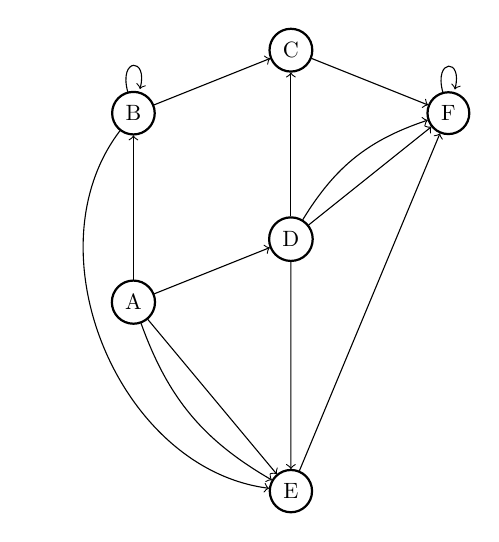
\begin{tikzpicture}[scale=0.8, transform shape]
	\begin{scope}[every node/.style={circle,thick,draw}]
		\node[] (A) at (0,0) {A};
    \node (B) at (0,3) {B};
    \node[] (C) at (2.5,4) {C};
		\node[] (D) at (2.5,1) {D};
    \node (E) at (2.5,-3) {E};
    \node (F) at (5,3) {F} ;
\end{scope}

\begin{scope}[
              every node/.style={fill=white,circle},
							every edge/.style={draw=black}]
							\path[->] (A) edge (B);
							\path[->] (B) edge (C);
							\path[->] (A) edge (D);
							\path[->] (D) edge (C);
							\path[->] (A) edge (E);
							\onslide<2>{\path[->] (A) edge[bend right=20] (E);}
							\path[->] (D) edge (E);
							\path[->] (D) edge (F);
							\onslide<2>{\path[->] (D) edge[bend left=20] (F);}
							\path[->] (C) edge (F);
							\path[->] (E) edge (F); 
							\path[->] (B) edge[bend right=60] (E); 
							\onslide<3>{\path[->] (B) edge[ loop above] (B);}
							\onslide<3>{\path[->] (F) edge[ loop above] (F);}
\end{scope}
\end{tikzpicture}

		\column{0.5\linewidth}
		\begin{itemize}
			\item A graph can also have a \textit{collection} of edges, rather than a set. We call this a \textit{multigraph}.
				
			\item This allows multiple edges between the same pair of nodes.
				
			\item Some versions also allow \textit{self-loops}.
				
			\item But in our course we mostly consider \alert{simple} graphs, where $E$ is a set and there are no self-loops.
		\end{itemize}
	\end{columns}
\end{frame}

%%%%%%%%%%%%%%%%%%%%%%%%%%%%%%%%%%%%%%%%%%%%%%%%%%%%%%%%%%%%%%%%%%%%%%
\begin{frame}
	\frametitle{Putting some edges together}
	\begin{columns}[T]
		\column{0.5\linewidth}
			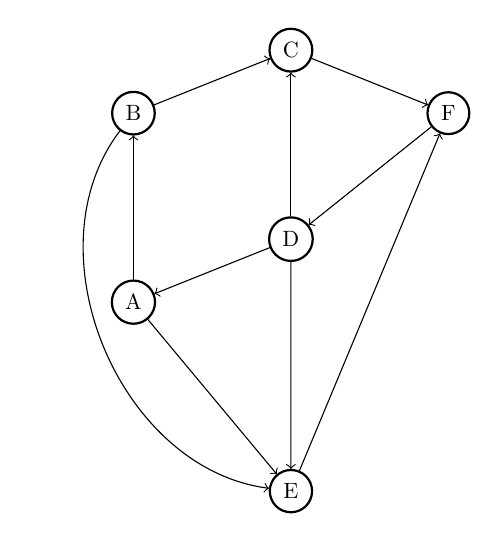
\begin{tikzpicture}[scale=0.8, transform shape]
	\begin{scope}[every node/.style={circle,thick,draw}]
		\node[] (A) at (0,0) {A};
    \node (B) at (0,3) {B};
    \node[] (C) at (2.5,4) {C};
		\node[] (D) at (2.5,1) {D};
    \node (E) at (2.5,-3) {E};
    \node (F) at (5,3) {F} ;
\end{scope}

\begin{scope}[
              every node/.style={fill=white,circle},
							every edge/.style={draw=black}]
							\path[->] (A) edge[] (B);
							\path[->] (B) edge[] (C);
							\path[->] (D) edge[] (A);
							\path[->] (D) edge (C);
							\path[->] (A) edge[] (E);
							\path[->] (D) edge (E);
							\path[->] (F) edge[] (D);
							\path[->] (C) edge[] (F);
							\path[->] (E) edge (F); 
							\path[->] (B) edge[bend right=60] (E); 
\end{scope}
\end{tikzpicture}

		\column{0.5\linewidth}
		\begin{itemize}
			\item A \textit{path} is a sequence of edges, connected to each other.
				
			\item Paths can even contain the same nodes twice.
			\item The path in \alert{red} starts at $A$ and ends at $E$.
				
			\item \textit{Cycles} are paths that start and end at the same vertex.
				
			\item Simple paths and simple cycles allow every vertex at most once (with the exception for a cycle, where the
				starting vertex is equal to the ending vertex).
		\end{itemize}
	\end{columns}
\end{frame}

%%%%%%%%%%%%%%%%%%%%%%%%%%%%%%%%%%%%%%%%%%%%%%%%%%%%%%%%%%%%%%%%%%%%%%
\begin{frame}
	\frametitle{Paths}
		\begin{itemize}
			\item A path $\pi$ is commonly denoted as a sequence of vertices (in simple graphs), or a sequence of edges (in
				multi-graphs).
				
			\item If denoted as a sequence of vertices, then $\pi$ is a path iff for every consecutive vertices $u,v$ in the
				sequence, $\{u,v\} \in E$.
				
			\item If denoted as a sequence of edges, then $\pi$ is a path iff for every consecutive edges $e,f$ in the
				sequence, $e=\{u,v\}, f=\{v,w\}$ for some $u,v,w \in V$.
				
			\item A cycle is a path $\pi = \{v_1, \dots, v_1\}$ (when denoted as a sequence of vertices).
				
			\item For a directed graph, we can also speak of \textit{directed paths} and \textit{directed cycles}.
		\end{itemize}
\end{frame}

%%%%%%%%%%%%%%%%%%%%%%%%%%%%%%%%%%%%%%%%%%%%%%%%%%%%%%%%%%%%%%%%%%%%%%
\begin{frame}
	\frametitle{The longest path}
	\begin{columns}[T]
		\column{0.5\linewidth}
			\begin{tikzpicture}[scale=0.8, transform shape]
	\begin{scope}[every node/.style={circle,thick,draw}]
		\node[] (A) at (0,0) {A};
    \node (B) at (0,3) {B};
    \node[] (C) at (2.5,4) {C};
		\node[] (D) at (2.5,1) {D};
    \node (E) at (2.5,-3) {E};
    \node (F) at (5,3) {F} ;
\end{scope}

\begin{scope}[>={Stealth},
              every node/.style={fill=white,circle},
							every edge/.style={draw=black,very thick}]
							\path[->] (A) edge[onslide=<3>{draw=red}] (B);
							\path[->] (B) edge[onslide=<3>{draw=red}] (C);
							\path[->] (D) edge (A);
							\path[->] (D) edge (C);
							\path[->] (A) edge (E);
							\path[->] (D) edge[onslide=<3>{draw=red}] (E);
							\path[->] (F) edge[onslide=<3>{draw=red}] (D);
							\path[->] (C) edge[onslide=<3>{draw=red}] (F);
							\path[->] (E) edge (F); 
							\path[->] (B) edge[bend right=60] (E); 
\end{scope}
\end{tikzpicture}

		\column{0.5\linewidth}
Longest path?
		
			How many vertices are part of the longest simple path in this graph?
			\begin{itemize}
				\item 4
				\item 5 
				\item 6
				\item 7
				\item I don't know.
			\end{itemize}
		
			In this case 6. \\
			Fun fact: this is actually a \alert{very very hard problem} that Computer Scientists cannot solve efficiently. More
			information on this when we discuss P vs NP.
	\end{columns}
\end{frame}

%%%%%%%%%%%%%%%%%%%%%%%%%%%%%%%%%%%%%%%%%%%%%%%%%%%%%%%%%%%%%%%%%%%%%%
\begin{frame}
	\frametitle{Finally we have reached the end}

Reachability:
			\begin{itemize}
				\item We say a node $v$ is \alert{reachable} from a node $u$ iff there is a (directed) path $\pi$ starting in
					$u$ and ending in $v$.
					
				\item A directed graph is \alert{strongly connected} if for any two vertices there is a directed path between them.
				\item In other words, if $\forall u,v \in V:$ $v$ is reachable from $u$.
					
				\item Finally then, a \alert{Directed Acyclic Graph (DAG)}  is a directed graph that has no cycles in it.
			\end{itemize}
\end{frame}

%%%%%%%%%%%%%%%%%%%%%%%%%%%%%%%%%%%%%%%%%%%%%%%%%%%%%%%%%%%%%%%%%%%%%%
\begin{frame}
	\frametitle{DAG or $\neg$DAG}
	
	\begin{columns}[T]
		\column{0.5\linewidth}
			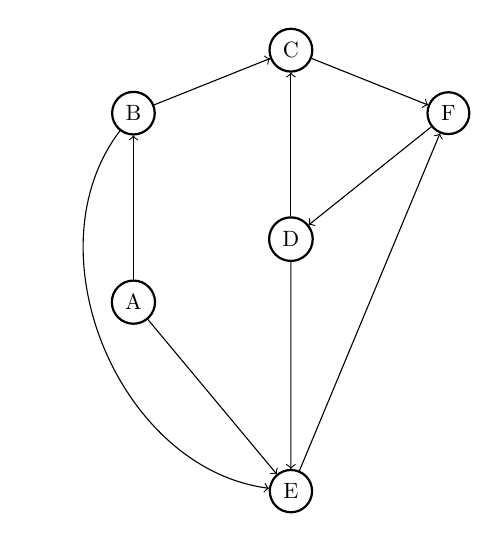
\begin{tikzpicture}[scale=0.8, transform shape]
	\begin{scope}[every node/.style={circle,thick,draw}]
		\node[] (A) at (0,0) {A};
    \node (B) at (0,3) {B};
    \node[] (C) at (2.5,4) {C};
		\node[] (D) at (2.5,1) {D};
    \node (E) at (2.5,-3) {E};
    \node (F) at (5,3) {F} ;
\end{scope}

\begin{scope}[
              every node/.style={fill=white,circle},
							every edge/.style={draw=black}]
							\path[->] (A) edge[] (B);
							\path[->] (B) edge[] (C);
							\path[->] (D) edge (C);
							\path[->] (A) edge (E);
							\path[->] (D) edge[] (E);
							\path[->] (F) edge[] (D);
							\path[->] (C) edge[] (F);
							\path[->] (E) edge (F); 
							\path[->] (B) edge[bend right=60] (E); 
\end{scope}
\end{tikzpicture}

		\column{0.5\linewidth}
		
			Is this a DAG?
			\begin{itemize}
				\item Yes
				\item No, but if we add one edge then it is.
				\item No, but if we remove one edge then it is.
				\item No, and we need to remove more than one edge to make it one.
				\item I don't know.
			\end{itemize}
		
			Just remove the edge $(F,D)$.
	\end{columns}
\end{frame}

%%%%%%%%%%%%%%%%%%%%%%%%%%%%%%%%%%%%%%%%%%%%%%%%%%%%%%%%%%%%%%%%%%%%%%
\begin{frame}
	\frametitle{Depth-first Search}

			\begin{itemize}
				\item Imagine you are walking in a labyrinth.
							\item 	You bring a some paint and a piece of rope, tie it to the entrance and start walking. Here's what you do:
			
			\begin{itemize}
				\item If we come to a cross-way, just pick one direction.
					
				\item If we get to a dead-end, we back up to the last cross-way. Now use the paint to cross out the way you just
					went.
					
				\item Repeat until you find the exit.
			\end{itemize}
		\end{itemize}	
	
\end{frame}

%%%%%%%%%%%%%%%%%%%%%%%%%%%%%%%%%%%%%%%%%%%%%%%%%%%%%%%%%%%%%%%%%%%%%%

\begin{frame}[fragile]
	\frametitle{An implementation}
	

	
	\begin{columns}[T]
		\column{0.455\linewidth}
		What is the run time of this algorithm?
		\begin{itemize}
			\item $\Theta(|V|)$
			\item $\Theta(|E|)$
			\item $\Theta(|V| + |E|)$
			\item $\Theta(|V|\times|E|)$
		\end{itemize}
		\column{0.455\linewidth}
		
			Worst-case we consider every vertex once and ever edge once.
	\end{columns}
	
	\begin{lstlisting}{DFS}
	Function{DFS}{$v$}
		For{each outgoing edge $e=(v,u)$ of $v$}
			If{$u$ is not visited yet}
				State mark $u$ as visited
				State Call{DFS}{$u$}
			EndIf
		EndFor
	EndFunction
	Comment{Ensure that $v$ is marked as visited before starting}
\end{lstlisting}
\end{frame}

%%%%%%%%%%%%%%%%%%%%%%%%%%%%%%%%%%%%%%%%%%%%%%%%%%%%%%%%%%%%%%%%%%%%%%
\begin{frame}
	\frametitle{Let's apply it!}

		So lets draw a graph on the smart board and then apply DFS on it!
\end{frame}

%%%%%%%%%%%%%%%%%%%%%%%%%%%%%%%%%%%%%%%%%%%%%%%%%%%%%%%%%%%%%%%%%%%%%%
\begin{frame}
	\frametitle{But what if I don't like recursion\dots}

		How could we get rid of the recursion?
		\begin{itemize}
			\item Adding nodes to explore to a set and taking the next node to visit randomly from the set.
			\item Adding nodes to explore to a stack and taking the next node to visit from the top of the stack.
			\item Adding nodes to explore to a queue and taking the next node to visit from the front of the queue.
			\item I don't know.
		\end{itemize}
\end{frame}

%%%%%%%%%%%%%%%%%%%%%%%%%%%%%%%%%%%%%%%%%%%%%%%%%%%%%%%%%%%%%%%%%%%%%%
\begin{frame}[fragile]
	\frametitle{An implementation}
	
	\begin{lstlisting}
		Function{DFS}{$v$}
			State $s gets$ empty Stack
			State $s$.push($v$)
			State mark $v$ as visited
			While{$s$ is not empty}
				State cur $gets$ $s$.pop()
				For{each outgoing edge $e=(\text{cur},u)$ of $\text{cur}$}
					If{$u$ is not visited yet}
						State mark $u$ as visited
						State $s$.push($u$)
					EndIf
				EndFor
			EndWhile
		EndFunction
	\end{lstlisting}
\end{frame}

%%%%%%%%%%%%%%%%%%%%%%%%%%%%%%%%%%%%%%%%%%%%%%%%%%%%%%%%%%%%%%%%%%%%%%
\begin{frame}
	\frametitle{So what can we do with this?}

			\begin{itemize}
				\item Find a path between vertices, if one exists! %(Including finding your way home to Haarlem.)
					
				\item Test if $G$ is a connected graph.
					
				\item Find a cycle in $G$ if there is one (that $v$ is a part of).
			\end{itemize}
			
\end{frame}

%%%%%%%%%%%%%%%%%%%%%%%%%%%%%%%%%%%%%%%%%%%%%%%%%%%%%%%%%%%%%%%%%%%%%%
\begin{frame}[fragile]
	\frametitle{What if we use a queue though?}
	
	
	\begin{lstlisting}
		Function{BFS}{$v$}
			State $s gets$ empty \alert{Queue}
			State $s$.enqueue($v$)
			State mark $v$ as visited
			While{$s$ is not empty}
				State cur $gets$ $s$.dequeue()
				For{each outgoing edge $e=(\text{cur},u)$ of $\text{cur}$}
					If{$u$ is not visited yet}
						State mark $u$ as visited
						State $s$.enqueue($u$)
					EndIf
				EndFor
			EndWhile
		EndFunction
	\end{lstlisting}
\end{frame}

%%%%%%%%%%%%%%%%%%%%%%%%%%%%%%%%%%%%%%%%%%%%%%%%%%%%%%%%%%%%%%%%%%%%%%
\begin{frame}[fragile]
	\frametitle{So what does this BFS do?}

		\begin{itemize}
		\item We crawl over the graph, layer by layer.
		\item First we check all vertices at distance $1$ from our starting point.
		\item Then all vertices at distance $2$.
		\item Etc. Etc.
		\end{itemize}	
		So lets draw a graph on the smart board and then apply BFS on it!
\end{frame}


%%%%%%%%%%%%%%%%%%%%%%%%%%%%%%%%%%%%%%%%%%%%%%%%%%%%%%%%%%%%%%%%%%%%%%
\begin{frame}
	\frametitle{Jobs to do!}

Tons of things to do: 	I have a bunch of things to do, that depend on each other. My question is, what order can I do them in so that all
		dependencies are met?
	
	\begin{columns}[T]
		\column{0.455\linewidth}
			I need to do the following things:
			\begin{itemize}
				\item Create an exam
		
				\item Have the exam proof read
				\item Print the exam
		
				\item Make the answer sheet
				\item Print the answer sheet
		
				\item Bring everything to location
			\end{itemize}
		\column{0.455\linewidth}
			\begin{itemize}
				\item Lets make that into a graph!
				\item Tasks become vertices.
				\item And dependencies become edges.
			\end{itemize}	
	\end{columns}
\end{frame}

%%%%%%%%%%%%%%%%%%%%%%%%%%%%%%%%%%%%%%%%%%%%%%%%%%%%%%%%%%%%%%%%%%%%%%
\begin{frame}
	\frametitle{Now what do we need?}
	
A topological ordering: 
			A topological ordering of the vertices $V$ in a \textit{directed} graph, is an ordering $v_1, \dots, v_n$ such
			that $e=(v_i,v_j)$ with $i < j$ for all $e \in E$.

		
			A graph $G$ has a topological ordering if and only if it is a DAG.
		
		\begin{proof}
			(first part) Suppose $G$ has a topological ordering.\\
			
			We now use a proof by contradiction. Assume there is a cycle (i.e. it is no DAG). That means there is a cycle
			$(v_x, v_y), \dots (v_w, v_x)$. But if it has a topological ordering, then $x < y < w < x$, which is clearly not
			possible.\\
			
			(second part) A little harder... Let's make an algorithm!
		\end{proof}
\end{frame}

%%%%%%%%%%%%%%%%%%%%%%%%%%%%%%%%%%%%%%%%%%%%%%%%%%%%%%%%%%%%%%%%%%%%%%
\begin{frame}
	\frametitle{The idea}

			\begin{itemize}
				\item 
					If $G$ is acyclic, there must be some vertex without incoming edges.
				\item
					We can start with this one, add it to the topological ordering and remove its outgoing edges.
				\item
					Now repeat!
			\end{itemize}

				Why must this be the case?
\end{frame}

%%%%%%%%%%%%%%%%%%%%%%%%%%%%%%%%%%%%%%%%%%%%%%%%%%%%%%%%%%%%%%%%%%%%%%
\begin{frame}[fragile]
	\frametitle{Lets code it!}
	
	\begin{columns}[T]
		\column{0.555\linewidth}
		{
	\small
	\begin{lstlisting}
		Function{Topo}{$G$}
			State order $gets$ empty list
			State q $gets$ empty queue
		
			State $v gets$ a random vertex with $\mathit{indeg}(v) = 0$.
			State q.enqueue($v$)
		
			While{q is not empty}
				State $v gets$ q.dequeue()
				State order.append($v$)
		
				For{each outgoing edge $e=(v,u)$ of $v$}
					State $G$.remove(e)
		
					If{$\mathit{indeg}(u) == 0$}
						State q.enqueue($u$)
		
					EndIf
				EndFor
			EndWhile
		EndFunction
	\end{lstlisting}
}
			
		\column{0.405\linewidth}
				\begin{itemize}
					\item If we implement this efficiently\dots
						
					\item Then finding the first vertex is $\Theta(|V|)$
						
					\item We then consider all vertices at most once: $\Theta(|V|)$
						
					\item We also remove all edges at most once (which our map-based implementation can do in expected
						$\Theta(1)$): $\Theta(|E|)$.
					\item All-in-all: $\Theta(|V| + |E|)$.
				\end{itemize}	
		
	\end{columns}
\end{frame}

%%%%%%%%%%%%%%%%%%%%%%%%%%%%%%%%%%%%%%%%%%%%%%%%%%%%%%%%%%%%%%%%%%%%%%
\begin{frame}
	\frametitle{One closing remark}
	
One important difference
				\begin{itemize}
					\item Both DFS/BFS and the topological ordering give an order of the nodes.
					\item But is there a difference? (Other than the order in which they are returned?)
				\end{itemize}

		
				\begin{itemize}
					\item DFS/BFS require a starting node! And give different results (not necessarily the whole graph) when starting from
			different nodes.
								\item 
			Topological orderings are Graph properties, not depending on a specific vertex!
				\end{itemize}
\end{frame}

%%%%%%%%%%%%%%%%%%%%%%%%%%%%%%%%%%%%%%%%%%%%%%%%%%%%%%%%%%%%%%%%%%%%%%
\begin{frame}
	\frametitle{Implementing a graph}

Implementations. There are many options:
		\begin{itemize}
			\item Edge List: just keep one list of all edges of the graph.
				
			\item Adjacency List: for every vertex, keep a list of all incident edges.
				
			\item Adjacency Matrix: a massive 2D array of size $|V|\times |V|$. Every entry can hold an edge.
				
			\item Adjacency Map: Just the best option. We will discuss this one now.
		\end{itemize}
\end{frame}

%%%%%%%%%%%%%%%%%%%%%%%%%%%%%%%%%%%%%%%%%%%%%%%%%%%%%%%%%%%%%%%%%%%%%%
\begin{frame}
	\frametitle{Vertex class}
	
	\begin{columns}[T]
		\column{0.505\linewidth}
			\lstinputlisting[basicstyle=\tiny\ttfamily, lastline=23	]{src/vertex.py}
		\column{0.455\linewidth}
		\begin{itemize}
			\item Initialise a Vertex, with a \texttt{dict} to hold neighbours.
			\item It is now $O(1)$ to add an edge, but this only works for \textit{simple} graphs.
			\item Getting all neighbours is $O(\mathit{deg}(v))$, which is the best we can get.
			\item A generator that allows us to iterate over the (outgoing) edges of this node.
			\item And we can make more functions as need be.
		\end{itemize}
			
	\end{columns}
\end{frame}

%%%%%%%%%%%%%%%%%%%%%%%%%%%%%%%%%%%%%%%%%%%%%%%%%%%%%%%%%%%%%%%%%%%%%%
\begin{frame}
	\frametitle{Graph class}
	
	\begin{columns}[T]
		\column{0.505\linewidth}
			\lstinputlisting[basicstyle=\tiny\ttfamily]{src/graph.py}
		\column{0.455\linewidth}
		\begin{itemize}
			
			\item A graph is just a bunch of vertices now.
				
			\item Adding a vertex is adding it to the dictionary.
			\item Using a dictionary allows $O(1)$ retrieval based on node name (e.g.\ Amsterdam)
				
			\item Getting all vertices, is just all values from the list.
		\end{itemize}
			
	\end{columns}
\end{frame}

%%%%%%%%%%%%%%%%%%%%%%%%%%%%%%%%%%%%%%%%%%%%%%%%%%%%%%%%%%%%%%%%%%%%%%
\begin{frame}
	\frametitle{Rail networks}
	
Questions to ask:
				The NS maintains a large network of railroads in the Netherlands. There are many questions related to this:
				\begin{itemize}
					\item What cities can you reach by train?
						
					\item What is the quickest way to get from A to B?
						
					\item What is the best way to connect new stations to the network?
						
					\item How can we quickly tour the entire country?
				\end{itemize}
Traversals: 	This we can figure out by traversing the graph, which we will do today.

Shortest path algorithms:	

				\begin{itemize}
					\item This we can figure out by using a shortest path algorithm (next Monday).
					\item This we can figure out by using a Minimum Spanning Tree (next Tuesday).
			\end{itemize}
TSP: This we cannot figure out! It's called the Travelling Salesman Problem (Monday two weeks from now)
\end{frame}

%%%%%%%%%%%%%%%%%%%%%%%%%%%%%%%%%%%%%%%%%%%%%%%%%%%%%%%%%%%%%%%%%%%%%%
\begin{frame}
	\frametitle{Summary}

			This implementation is better than all others (that you can find in the book), tomorrow we will see to what extent you can
			reproduce these ideas in the tutorial.
		
		\begin{tabular}{c | c}
		Operation & Time complexity \\
		\midrule
		$|V|$ & $\Theta(1)$ \\
		$|E|$ & $\Theta(|V|)$\footnote{But we could make this $\Theta(1)$} \\
		
		\texttt{degree(v)} & $\Theta(1)$ \\
		\texttt{neighbours(v)} & $\Theta(\mathit{deg}(v))$ \\
		
		\texttt{add\_vertex(v)} & $\Theta(1)$ \\
		\texttt{add\_edge(v)} & $\Theta(1)$ \\
		
		And a bunch more & See the book if you want\\
		\end{tabular}
\end{frame}

